\documentclass{article}

\usepackage[T1]{fontenc} % add special characters (e.g., umlaute)
\usepackage[utf8]{inputenc} % set utf-8 as default input encoding
\usepackage{ismir,amsmath,cite,url}
\usepackage{graphicx}
\usepackage{color}
\usepackage{lineno}
\linenumbers

\DeclareMathOperator*{\argmax}{arg\,max}

% ------
\title{
Melody transcription via generative pre-training
%A fresh look at melody transcription
}

\threeauthors
  {First Author} {Affiliation1 \\ {\tt author1@ismir.edu}}
  {Second Author} {\bf Retain these fake authors in\\\bf submission to preserve the formatting}
  {Third Author} {Affiliation3 \\ {\tt author3@ismir.edu}}

% For the author list in the Creative Common license, please enter author names. 
% Please abbreviate the first names of authors and add 'and' between the second to last and last authors.
\def\authorname{F. Author, S. Author, and T. Author}

% Optional: To use hyperref, uncomment the following.
\usepackage[bookmarks=false,pdfauthor={\authorname},pdfsubject={\papersubject},hidelinks]{hyperref}
% Mind the bookmarks=false option; bookmarks are incompatible with ismir.sty.

\sloppy % please retain sloppy command for improved formatting

% My dependencies
\usepackage{booktabs}
\usepackage{cleveref}
\usepackage{amsfonts}
\usepackage{amssymb}

% My macros
\newcommand{\madmom}{\texttt{madmom}}
\newcommand{\mel}{Mel}
\newcommand{\mtthree}{MT3}
\newcommand{\jukebox}{Jukebox}
\newcommand{\hooktheory}{HookTheory}
\newcommand{\rwc}{RWC-MDB}
\newcommand{\sheetsage}{Sheet Sage}
\newcommand{\fone}{\texttt{F1}}
\newcommand{\fnot}{F0}
\newcommand{\Beatpooling}{Beat-wise resampling}
\newcommand{\beatpooling}{beat-wise resampling}

\newcommand{\cd}[1]{{\textcolor{blue}{[CD: #1]}}}
\newcommand{\jt}[1]{{\textcolor{magenta}{[JT: #1]}}}
\newcommand{\pl}[1]{\textcolor{red}{[PL: #1]}}
\newcommand{\todo}[1]{\textcolor{red}{[TODO: #1]}}
\newcommand\john[1]{\textcolor{magenta}{[JT: #1]}}

\interfootnotelinepenalty=10000

\begin{document}

\maketitle

\begin{abstract}
% Melody is a fundamental aspect of music perception. 
\john{abstract could be sharpened (how much can we change without complaints?)}
While even those without musical training can intuitively recognize the melody of a song by ear, 
it remains an open challenge in MIR to reliably detect the notes of the melody present in an arbitrary music recording. 
A key challenge in \emph{melody transcription} is building methods which can handle broad audio containing any number of instrument ensembles and musical genres. 
To confront this challenge, we leverage recent advancements in generative modeling of broad music audio, thereby improving performance on melody transcription by 
% (RWC All) .744 vs .631 = 17.9%
% (Hookthr) .615 vs .514 = 19.6%
% (RWC Vox) .786 vs .621 = 26.6%
up to $27$\% 
relative to conventional approaches. 
Another obstacle in melody transcription is a lack of training data---we collect, align, and release a new dataset consisting of $50$ hours of crowdsourced melody annotations for popular music. 
% (RWC Vox) 0.786 vs 0.462 = 70%
% (RWC All) 0.744 vs 0.420 = 77%
The combination of generative pre-training and a new dataset for this task results in up to $77\%$ stronger performance on melody transcription relative to the strongest available baseline. 
By pairing our new melody transcription approach with solutions for beat detection, key estimation, and chord recognition, 
we build a system capable of transcribing human-readable lead sheets directly from music audio.\footnote{Sound examples: \url{https://dblblnd.github.io/ismir22} \\
Demo / dataset explorer: \url{https://colab.research.google.com/drive/1yzD3wRCjXkuSfDRUtt_daaGFitj5L88l}\label{sound_examples}}
\end{abstract}

\section{Introduction}\label{sec:introduction}

In the Western music canon, 
%(and especially in popular music), 
\emph{melody} is a defining characteristic of musical composition. 
Even those without formal musical training can often effortlessly recognize a melody within a complex mixture of sounds, 
a ubiquitous skill which forms a pillar of our collective musical experience. %experience. 
Because of the significance of melody to music perception, 
the ability to automatically \emph{transcribe} the melody notes present in an arbitrary recording 
could enable numerous applications in 
% TODO: performance?
interaction~\cite{ryynanen2008accompaniment}, 
education~\cite{droe2006music}, 
informatics~\cite{bainbridge1999towards}, 
retrieval~\cite{ghias1995query}, 
source separation~\cite{ewert2014score},
and even generation~\cite{hawthorne2019enabling}.
Despite the potential benefits, 
reliable melody transcription remains an open challenge in MIR.

The relative lack of progress on melody transcription is perhaps counterintuitive when compared to the considerable progress on seemingly more difficult tasks like piano transcription~\cite{sigtia2016end,hawthorne2017onsets}.
%and chord recognition~\cite{humphrey2012rethinking,boulanger2013audio}. 
This circumstance stems from two primary factors. 
First, unlike in piano transcription, melody transcription involves operating on \emph{broad}
% CHRIS: I like broad slightly more I think
%\john{diverse?} 
audio mixtures from arbitrary instrument ensembles and genres. 
% CHRIS: I think the following are indeed reasons that melody transcription is hard, but they don't map as cleanly onto our contributions
%Second, unlike in chord recognition, melody transcription involves isolating the notes from a single instrument voice (recognized to be the melodic voice) within the mixture. 
%Second, melody transcription involves not only detecting notes but also identifying which of those notes constitutes the melody, which may require modeling the nuances of human music perception. 
Second, there is a deficit of training data for melody transcription, which particularly impedes the deep learning approaches central to recent improvements on other transcription tasks. 

\begin{figure}
    \centering
    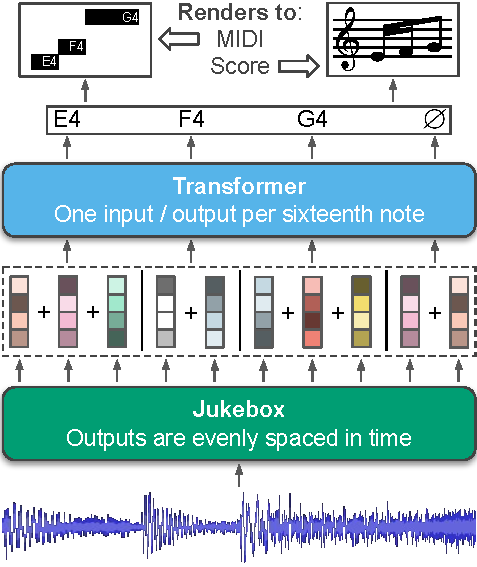
\includegraphics[width=8.1cm]{figs/fig1.pdf}
    \caption{
Our melody transcription approach involves 
(1)~extracting audio representations from Jukebox~\cite{dhariwal2020jukebox}, a generative model of music, 
(2)~averaging these representations across time to their nearest sixteenth note (dashed outline---uses \madmom{}~\cite{bock2016joint,bock2016madmom} for beat detection),
and
(3)~training a Transformer~\cite{vaswani2017attention} to detect note onsets (or absence thereof) per sixteenth note. 
Outputs can be rendered to MIDI (by mapping beats back to time) or a score.
}
 \label{fig:fig1}
\end{figure}

To overcome the challenge of transcribing broad audio, in this work we leverage representations from Jukebox~\cite{dhariwal2020jukebox}, a large-scale generative model of music audio pre-trained on $1$M songs~(\Cref{fig:fig1}). 
In~\cite{castellon2021calm}, Castellon~et~al.\ demonstrate that internal representations from Jukebox are useful for improving performance on a wide variety of MIR tasks. 
When used as input features to a Transformer model~\cite{vaswani2017attention}, representations from Jukebox outperform conventional spectrogram features used for melody transcription by 
% (RWC All) .744 vs .631 = 17.9%
% (Hookthr) .615 vs .514 = 19.6%
% (RWC Vox) .786 vs .621 = 26.6%
up to $27$\% (relative). 
% CHRIS: This was written conservatively because but could potentially be broadened... this may be the first time transfer learning has ever been used for transcription or any time-varying MIR task (though MT3 may be one instance)
To the best of our knowledge, this is the first evidence that representations learned through generative modeling are useful for time-varying MIR tasks like transcription, as opposed to the song-level tasks (e.g.~tagging, genre detection) examined in~\cite{castellon2021calm}.

\todo{First paragraph all about data and overcoming alignment challenges, second paragraph all about modeling wins}

%\john{Weak topic sentence. And this paragraph is kind of all over the place}
%To support this and future work on melody transcription, 
To address the data deficit for melody transcription, 
we release a new dataset containing $50$ hours of melody annotations 
%collected 
derived 
from \hooktheory.\footnote{\url{https://www.hooktheory.com/theorytab}} 
This dataset contains annotations for a broad audio: 
$13$k unique recordings representing a wide variety of instruments and genres. 
% This dataset contains $50$ hours of annotated melodies and harmonies (as chord names) aligned with audio recordings available on YouTube. 
%to aid chord recognition research. 
By training Transformer models on this new dataset using representations from Jukebox as input, we are able to improve overall performance on melody transcription by 
% 0.786 vs 0.462 = 70%
% 0.744 vs 0.420 = 77%
up to $77$\% 
relative to the strongest available baseline. 
% We also release all code and models needed to precisely reproduce all of our evaluations,\footnote{Released upon publication} facilitating comparison in future work even as some audio inevitably disappears from YouTube.

%\john{Maybe too many details? Content of this and previous paragraph might benefit from reorg/streamlining}
% CHRIS: I agree that this information feels a little verbose for an intoduction, but I think it's necessary to contextualize Figure 1. Another option is to obscure the beat pooling from Figure 1, but I think Figure 1 would then be too vague :/. Tricky situation
Because this new dataset has imprecise \emph{alignments} between the audio and melody annotations,
we also propose a new method for training transcription models in the presence of such alignments.
%imprecise audio-to-score alignments. 
% Existing transcription methods were largely designed for domains where perfect alignments are readily available, e.g.,~a Disklavier yields piano transcription data with perfect alignment. 
% The alignments in \hooktheory{} are not precise enough to facilitate effective transcription when adopting these methods off-the-shelf. 
% To address this, we propose a new method which  
Our approach 
involves aggregating input features (evenly spaced in time) into proxy features representative of individual sixteenth notes (evenly spaced in beats), 
thereby smoothing over alignment jitter. 
We train models on these beat-based features, 
which has a secondary benefit of enabling simple conversion from raw model outputs to human-readable scores (\Cref{fig:fig1}).

%\textbf{Contributions.} 
A summary of our primary \textbf{contributions} is as follows:
\begin{itemize}
    \item We show that representations from generative models can improve melody transcription (\Cref{sec:experiments}).
    \item We collect, align, and release a new dataset with $50$ hours of melody and chord annotations (\Cref{sec:dataset}).
    \item We propose a method for training transcription models on data with imprecise alignment (\Cref{sec:beatpool}).
    \item As a downstream application of our melody transcription approach, we build a system which can transcribe music audio into lead sheets (\Cref{sec:sheetsage}).
\end{itemize}

\section{Related work}\label{sec:related}

Melody transcription is closely related to but distinct from the task of \emph{melody extraction}, originally referred to as predominant fundamental frequency (\fnot) estimation~\cite{goto1999real,goto2004real}. 
Melody extraction has received significant interest from the MIR community over the last two decades (see~\cite{salamon2014melody,rao2022melody} for comprehensive reviews), 
and is the subject of an annual MIREX competition~\cite{downie2014ten}. 
Melody extraction may be a component of a melody transcription pipeline in combination with a strategy to segment \fnot{} into notes~\cite{salamon2015midi,nishikimi2016musical,nishikimi2017scale}---we directly compare to such a pipeline in \Cref{sec:exp2}.

Compared to melody extraction, melody transcription has received considerably less attention. 
Earlier efforts use sophisticated DSP-based pipelines~\cite{paiva2004auditory,paiva2005detection,ryynanen2008automatic,weil2009automatic}---unfortunately none of these methods provide code, though~\cite{ryynanen2008automatic} provides example transcriptions which we use to facilitate direct comparison. 
A more recent effort uses ground truth chord labels as extra information to improve melody transcription~\cite{laaksonen2014automatic}---in contrast, our method does not require extra information. 
Another line of work seeks to transcribe solo vocal performances into notes~\cite{mauch2015computer,nishikimi2020bayesian,nishikimi2021audio}. 
As singing voice often carries the melody in popular music, we directly compare to a baseline which firsts isolates the vocals (using~\cite{hennequin2020spleeter}) and then transcribes them.

Polyphonic music transcription is another related task which involves transcribing \emph{all} of the notes present in a recording (not just the melody).
This task has its own MIREX contest (Multiple Fundamental \fnot{} Estimation) alongside a growing collection of supervised training data resources \cite{benetos2013automatic,thickstun2017learning,hawthorne2019enabling,manilow2019cutting}. 
The similarity of the polyphonic and melody transcription problems motivates us to experiment with representations learned by a polyphonic system---specifically, MT3 \cite{gardner2021mt3}---for melody transcription.

\section{Task definition}
\label{sec:task}

We define melody transcription as the task of converting a music recording into a \emph{monophonic} (non-overlapping) sequence of \emph{notes} which constitute its melody.\footnote{Melody is difficult to precisely define---here we adopt an implicit definition based on a dataset of crowdsourced melody annotations.} Given a music recording $\bm{a}$ of length $T$, our task is to 
%generate 
uncover 
the sequence of $N$ notes~${\bm{y} = [\bm{y}_1,\dots,\bm{y}_N}]$ that represent the melody of $\bm{a}$.  For many MIR tasks, including transcription, it can be convenient to work with \emph{features} of audio ${\bm{X} = \texttt{Featurize}(\bm{a})}$, rather than the raw waveform $\bm{a}$. 
Hence, a melody transcription algorithm is a procedure that maps featurized audio to notes, i.e.~${\bm{y} = \texttt{Transcribe}(\bm{X})}$. 

% CHRIS: Cutting for space
% \begin{figure}
%     \centering
%     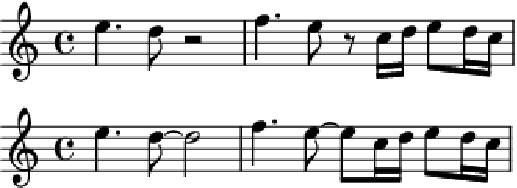
\includegraphics[width=8.1cm]{figs/heuristic_offsets.pdf}
%     \caption{
% The same note onsets engraved with ground truth~(top) vs. heuristic~(bottom) offsets. 
% We argue that onset prediction suffices for producing melody transcriptions that are both recognizable and readable. 
% }
%  \label{fig:heuristic_offsets}
% \end{figure}

Canonically, a musical note consists of an onset time, a musical pitch, and an offset time. 
However, in this work  
%(and as in~\cite{laaksonen2014automatic}) 
we disregard offsets and define a note to be a pair $\bm{y}_i = (t_i,n_i)$ consisting of an onset time~${t_i \in [0,T)}$ and discrete musical pitch~${n_i \in \mathbb{V} = \{\text{A0}, \ldots, \text{C8}\}}$.
We ignore offsets for 
%three 
two reasons. 
First, accurate offsets have been found to be considerably less important for human perception of transcription quality compared to accurate onsets~\cite{ycart2020investigating}. 
Second, in our dataset,
a heuristically-determined offset is identical to the ground truth offset for $89\%$ of notes.\footnote{The heuristic we adopt sets the offset of one note equal to the onset of the next, i.e., it assumes the melody is legato.}
% Finally, we argue intuitively that onsets and pitches suffice for both recognizing and reading melodies---see~\Cref{fig:heuristic_offsets} for an example.

Formally, a musical audio recording of length~$T$ seconds sampled at rate~$f_s$ is a vector~${\bm{a} \in \mathbb{R}^{Tf_s}}$. 
A featurization of audio ${\bm{X} \in \mathbb{R}^{Tf_k \times d}}$ is a matrix of $d$-dimensional features of audio, sampled uniformly at some rate ${f_k \ll f_s}$ (for example, $\bm{X}$ could be a spectrogram).
Intuitively, the function ${\texttt{Featurize} : \mathbb{R}^{Tf_s} \to \mathbb{R}^{Tf_k \times d}}$ defined by ${\bm{a} \mapsto \bm{X}}$ maps 
%scalar audio samples 
raw audio 
to a feature representation more conducive to learning. 
A melody of length $N$ is a sequence of notes 
% CHRIS: Should this be raised to the N? JOHN: nope, \bm{y} \in \mathcal{N}^N but y_1,\dots,y_N \in \mathcal{N}
$\bm{y} = [\bm{y}_1,\dots,\bm{y}_N] \in \mathbb{Y}^N$
%\pl{add []} \pl{a bit confusing, should be raised to $N$ power since that's the type of the sequence not an element}
consisting of onset-pitch pairs ${\bm{y}_i = (t_i,n_i)} \in \mathbb{Y} = \mathbb{R}^+ \times \mathbb{V}$ where ${t_i < t_j}$ if ${i < j}$. Given a featurization $\bm{X}$, the melody transcription task is to construct a transcription algorithm ${\texttt{Transcribe} : \mathbb{R}^{Tf_k \times d} \to \mathbb{Y}^N}$ such that ${\bm{X} \mapsto \bm{y}}$.


%Hence, 
%\begin{gather*}
%    %\bm{a} &= a_1, \ldots, a_S, \text{where}~S %= Tf_s \\
%    \bm{y} = y_1, \ldots, y_N, \\
%    \text{where}~y_i = (t_i, n_i), t_i \leq T, %\text{and}~n_i \in \{\text{A0}, \ldots, %\text{C8}\}.
%\end{gather*}
%\todo{Remove high-dimensionality quip, replace with specifics (spectrograms)... for MIR tasks, often better to work with features rather than raw audio...}
%\john{Not sure high-dimensionality is the right motivation here}

%To handle the high dimensionality of audio, transcription algorithms typically extract features $\bm{X}$ (a matrix) from audio, which are sampled at ${f_k \ll f_s}$:
%\begin{gather*}
%    \text{Extract}(\bm{a}) = \bm{X} = \bm{x}_1, %\ldots, \bm{x}_M, \\ 
%    \text{where}~M = Tf_k, \text{and}~\bm{x}_i %\in \mathbb{R}^d.
%\end{gather*}

\subsection{Evaluation}
\label{sec:eval}

% CHRIS: This maps cleanly onto our contributions (standardized evaluation and new datasets), but may be too snarky for paragraph 2
%Finally, we argue that a historical focus on the important but disparate task of melody \emph{extraction}---detecting the time-varying fundamental frequency of the melody as opposed to its discrete notes---has led to a lack of work on transcription and systemic issues in evaluation.
% \john{Leading with an MIR implementation of F1 is a little confusing, especially since it is not typically applied to this task (you are defining the task, right?)}
% CHRIS: Reworked to clarify that this is a departure from melody extraction

%\john{Maybe lead with why we need to invent our own metrics?}
To evaluate a melody transcription method $\texttt{Transcribe}$, 
we adopt a standard metric commonly used for evaluation in polyphonic music transcription tasks, namely,  ``onset-only notewise F-measure''~\cite{ycart2020investigating}. 
This metric scores an estimated transcript $\texttt{Transcribe}(\bm{X})$ by first matching its note onsets to those in the reference $\bm{y}$ with $50$ms of tolerance, and then computes a standard \fone{} score where an estimated note is treated as correct if it is the same pitch as its matched reference note. 
% \begin{equation*}
%      \text{\fone} : f(\bm{X}), y \mapsto [0, 1].
% \end{equation*}
This ``notewise'' metric represents a departure from the ``frame-based'' metrics typically used to evaluate melody extraction algorithms---Ycart~et~al.\ demonstrate in~\cite{ycart2020investigating} that this particular notewise metric correlates more strongly with human perception of transcription quality than any other common metric, including frame-based ones.

We make a slight modification to this notewise metric 
%to make it more appropriate for 
specific to 
the melody transcription setting: an estimate $\texttt{Transcribe}(\bm{X})$ may receive full credit if it is off by a fixed octave shift but otherwise identical to the reference. 
In downstream settings, melody transcriptions are likely to be used in an octave-invariant fashion, e.g.,~they may be shifted to read more comfortably in treble clef, or performed by singers with different vocal ranges. 
% Previous evaluations for melody extraction gave full credit for estimates with the right pitch class, ignoring octaves entirely (see~\cite{poliner2007melody} for a summary). 
% However we argue that this is overly permissive, as \emph{relative} octave information preserves intervals between notes, and thus may be critical to the identity of a melody. 
Hence, we modify the evaluation criteria by simply taking the highest score over octave shifted versions of the estimate:
\begin{equation*}
    \max_{\sigma \in \mathbb{Z}} \texttt{\fone}(\texttt{OctaveShift}(\texttt{Transcribe}(\bm{X}), \sigma), \mathbf{y}).
\end{equation*}
Henceforth, we refer to this octave-invariant metric as \fone. 

\vspace{-2mm}
\section{Dataset overview}
\label{sec:dataset}

A major obstacle to progress on melody transcription is the lack of a large volume of data for training. 
To the best of our knowledge, 
there are only two datasets available with annotations suitable for melody transcription: the RWC Music Database~\cite{goto2002rwc,goto2003rwc,goto2004development} (RWC-MDB), 
and a dataset labeled by Laaksonen~\cite{laaksonen2014automatic}. 
The former is larger but the annotations are inconsistent---Ryyn{\"a}nen~and~Klapuri note that only $8.7$ hours ($130$ songs) are usable for melody transcription~\cite{ryynanen2008automatic}, while the latter only contains $1.5$ hours. 

We derive a suitably large dataset for melody transcription using crowdsourced annotations from \hooktheory{}.\footnote{\hooktheory{} annotations are published under a \href{https://creativecommons.org/licenses/by-nc-sa/3.0/}{CC BY-NC-SA 3.0} license, which our dataset inherits.}
\hooktheory{} is a platform where users can easily create and share musical analyses of particular recordings hosted on YouTube, with Wikipedia-style editing. 
The dataset contains annotations for $22$k segments of $13$k unique recordings totaling $50$ hours of labeled audio. 
The audio content covers a wide range of genres---there is a skew towards pop and rock but many other genres are represented including EDM, jazz, and even classical. 
We create an artist-stratified $8$:$1$:$1$ split of the dataset for training, validation, and testing. 
The dataset also includes chord annotations which may facilitate chord recognition research.

While \hooktheory{} data has been used previously for MIR tasks like 
harmonization~\cite{chen2021surprisenet,yeh2021automatic}, 
chord recognition~\cite{jiang2019mirex}, and 
representation learning~\cite{jiang2020transformer}, 
making use of this platform for MIR is currently cumbersome. 
One obstacle is that the annotations are created via a ``functional'' interface, i.e.,~one which uses scale degrees and roman numerals relative to a key signature instead of absolute notes and chord names. 
In contrast, most MIR research favors absolute labels.
Hence, we convert annotations from this functional format to a simple (JSON-based) absolute format. 
One caveat is that the \hooktheory{} annotation interface uses a relative octave system, 
so there is no way to reliably map annotations to a ground truth octave.
Thus, melodies in our dataset also contain only relative octave information, consistent with the octave-invariant evaluation proposed in \Cref{sec:eval}.

\section{Methods}

As in state-of-the-art methodology for other areas of transcription~\cite{hawthorne2021sequence}, 
our approach to melody transcription involves training Transformer~\cite{vaswani2017attention} models to predict notes from audio features. 
However, our approach differs in two distinct ways to address to the challenges unique to melody transcription.
First, because melody transcription involves operating on broad audio, we leverage representations from pre-trained models as drop-in replacements for the handcrafted spectrogram features used as inputs to other transcription systems. 
Secondly, because alignments in our dataset are approximate, we propose a new strategy for training transcription models under such conditions.

\subsection{Pre-trained representations}
\label{sec:representations}

We explore representations from two different pre-trained models for use as input features to transcription models.
In~\cite{castellon2021calm}, Castellon~et~al.\ demonstrate that representations from \jukebox---a generative model of music audio pre-trained on $1$M songs---constitute general purpose features for MIR tasks, though notably they do not verify this claim for transcription. 
We adopt their approach to extract features from \jukebox{} ($f_k \approx 345$ Hz, $d = 4800$), however we pull representations from a deeper layer of \jukebox{} ($54$ vs. $36$), which Castellon~et~al.\ found to be more effective for note-aware tasks like key estimation. 

We also explore features from \mtthree~\cite{gardner2021mt3}, an encoder-decoder transcription model pre-trained on a multitude of different transcription tasks (though not melody transcription). 
For this model, we use the output of the encoder ($f_k = 125$ Hz, $d = 512$) as our feature representation. 
The two models have different trade-offs with respect to our setting: \jukebox{} was trained on audio similar to that found in our dataset but explores a different task (generative modeling), whereas \mtthree{} is pre-trained on transcription but for different audio domains. 

\subsection{Beat pooling}
\label{sec:beatpool}

\todo{Copied from intro. Need to integrate}
\john{Again too much detail} We also propose a new strategy for training transcription models in the presence of imprecise alignments. 
User annotations from \hooktheory{} have coarse alignments with the audio---users only provide the starting and ending timestamp of a segment. 
We use beat tracking to refine these alignments, but they are still not as precise as the flawless alignments found in other transcription datasets (e.g.,~piano transcription datasets captured using a Disklavier) which existing methods rely on. 
To address this, our approach involves aggregating input features (evenly spaced in \emph{time}) into proxy features which represent individual sixteenth notes (evenly spaced in \emph{beats}), 
which effectively smooths over alignment jitter. 
This approach has a secondary benefit of trivializing the process of converting output from the transcription model into a human-readable score format. %which is simpler for musicians to interpret compared to MIDI.

% Alignment
Despite our best efforts, the refined alignments in \hooktheory{} are still imprecise when compared to those found in datasets used by piano transcription methods. 
In initial experiments, we found that naively adopting methods designed for piano transcription~\cite{hawthorne2017onsets,hawthorne2021sequence} resulted in poor performance on our dataset and task.\footnote{Additionally, training models with an alignment-free approach~\cite{graves2006connectionist} also resulted in poor performance.} 
Hence, we designed a new approach for training models in the presence of approximate alignments. 

Our approach works by averaging all of the feature vectors (equally spaced in time) that are nearest to a particular sixteenth note into a single vector which acts as a proxy feature for that sixteenth note. 
For example, if a recording has a tempo of $120$ beats per minute, a sixteenth note represents $125$ ms of time, which would mean averaging across around $43$ feature vectors from \jukebox{} ($f_k \approx 345$ Hz). 
The intuition is that, while our beat tracked alignments may not be able to identify precisely where the ground truth onset occurs in these $43$ frames, we can be reasonably confident that it occurs \emph{somewhere} within them, and thus that information will be incorporated into the feature vector.
We refer to this strategy as \emph{beat pooling}.

\todo{John, I could use your eyeballs / refinement on this. One question is whether or not the 1-based indexing for beats makes this super confusing. Feel free to ask for clarification on anything}
Formally, for a segment of length $T$ seconds and $B$ beats, and an alignment function $a: [0, T] \mapsto [1, B]$, beat pooling yields a matrix $\hat{\bm{X}} = \hat{\bm{x}}_1, \ldots, \hat{\bm{x}}_{4B}$, where $\hat{\bm{x}}_i \in \mathbb{R}^d$, and
\begin{gather*}
\bm{\hat{x}}_i = \frac{1}{r_i - l_i} \sum_{j = l_i}^{r_i - 1} \bm{x}_j, \text{where} \\
l_i = \left\lfloor a \left(\frac{2i + 5}{8} \right) \cdot f_k \right\rfloor, \text{and}~
r_i = \left\lfloor a \left(\frac{2i + 7}{8} \right) \cdot f_k \right\rfloor.
\end{gather*}

\subsection{Training}

The output of our beat pooling approach ($\hat{\bm{X}}$) represents a sequence of features where a timestep is a sixteenth note, and constitutes the input to the transcription model we will train. 
Analogously, we also construct a sequence containing labels for each sixteenth note $\hat{\bm{y}} \in \mathbb{V}^{4B}$, where 
$\mathbb{V} = \{\varnothing, \text{A0}, \ldots, \text{C8}\}$.\footnote{This requires quantizing labels to the nearest sixteenth note. In practice, less than $1\%$ of notes are affected by this quantization, and $99\%$ of segments contain no affected notes.} 
This sequence indicates for each sixteenth note whether or not an onset occurs ($\varnothing$ if not, note name if so). 
Then, we can formulate melody transcription as an aligned sequence-to-sequence modeling problem and train models of the form $f_{\theta} : \mathbb{R}^{4B \times d} \mapsto \mathbb{R}^{4B \times |\mathbb{V}|}$ using a standard cross entropy loss. 

An additional challenge is that octave information is often incorrect in our dataset (see \Cref{sec:dataset}). 
Hence, we construct an octave-tolerant loss function by octave shifting the labels and backpropagating on whichever shift minimizes the loss:
\begin{equation*}
\operatorname*{min}_{\sigma \in \{-\alpha, \ldots, \alpha\}} \sum_{i=1}^{4B} \text{CrossEntropy}(f_{\theta}(\bm{\hat{X}})_i, \text{OctaveShift}(\hat{\bm{y}}_i, \sigma)). 
\end{equation*}
Here, $\alpha$ is an integer determining the number of possible shifts, and $\alpha = 0$ constitutes the standard cross entropy loss. 
In practice, we found $\alpha = 2$ produced the best results, while $\alpha > 3$ resulted in unstable training.


\begin{table}[t]
    \centering
    \begin{tabular}{lcc}
\toprule
Features & $d$ & \fone{} \\
\midrule
\mel{} & $229$ & $0.514$ \\
\mtthree{} & $512$ & $0.550$ \\
\jukebox{} & $4800$ & $\bm{0.615}$ \\
\midrule
\mel{}, \mtthree{} & $741$ & $0.548$ \\
\mel{}, \jukebox{} & $5029$ & $0.617$ \\
\mtthree{}, \jukebox{} & $5312$ & $0.622$ \\
\mel{}, \mtthree{}, \jukebox{} & $5541$ & $\bm{0.623}$ \\
\bottomrule
    \end{tabular}
    \caption{\hooktheory{} test set performance for Transformers trained with different features (top) and combinations (bottom). Features are complementary---combining all three yields highest performance---but marginally so compared to \jukebox{} alone.}
    \label{tab:hooktheory_test}
    \vspace{-3mm}
\end{table}

\section{Experiments}
\label{sec:experiments}

Here we describe our experimental protocol for training melody transcription models on the \hooktheory{} dataset. 
The purpose of these experiments is two-fold. 
First, we compare representations from different pre-trained models to handcrafted spectrogram features to determine if pre-training is helpful for the task of melody transcription (\Cref{sec:exp1}). 
Second, we compare our trained models holistically to other melody transcription baselines (\Cref{sec:exp2}).

All transcription models are encoder-only Transformers with the default hyperparameters from~\cite{vaswani2017attention}, 
except that we reduce the number of layers from $6$ to $4$ to allow models to be trained on GPUs with $12$GB of memory. 
During training, we select random slices from the annotated segments of up to $96$ beats or $24$ seconds in length (whichever is shorter). 
We train using our proposed loss function from~\Cref{sec:modeling} and perform early stopping based on max \fone{} score across thresholds $\tau$ on the validation set, using the best validation $\tau$ for testing. 
All models converge within $15$k steps or about a day on a single K40 GPU. 

\subsection{Comparing input features}
\label{sec:exp1}

We compare representations from \jukebox~\cite{dhariwal2020jukebox} and \mtthree~\cite{gardner2021mt3} (see~\Cref{sec:representations}) to handcrafted spectrogram features, 
which are commonly used by existing transcription methods.
Specifically, we compare to log-amplitude Mel spectrograms using the formulation from~\cite{hawthorne2017onsets} (${f_k \approx 31}$,~${d = 229}$). 
Because features may contain complementary information, we also experiment with all combinations of these three features. 
Note that our \beatpooling{} strategy allows for trivial combination of these features (by concatenation) despite their differing rates. 
In~\Cref{tab:hooktheory_test}, we report \fone{} (as described in~\Cref{sec:eval}) on the \hooktheory{} test set for all input features.

\begin{table}[t]
    \centering
    \begin{tabular}{lcc}
\toprule
Approach & \fone{} (All) & \fone{} (Vocal)\\
\midrule
MT3 Zero-shot~\cite{gardner2021mt3} & $0.133$ & $0.085$ \\
% TODO: This number is wrong... should be 0.224 and 0.2035
Melodia~\cite{salamon2014melody} + Segmentation & $0.201$ & $0.268$ \\
Spleeter~\cite{hennequin2020spleeter} + Tony~\cite{mauch2015computer} & $0.341$ & $\bm{0.462}$ \\
DSP + HMM~\cite{ryynanen2008automatic} & $\bm{0.420}$ & $0.381$ \\
\midrule
\mel{} + Transformer & $0.631$ & $0.621$ \\
\mtthree{} + Transformer & $0.701$ & $0.659$ \\
\jukebox{} + Transformer & $\mathbf{0.744}$ & $\mathbf{0.786}$ \\
\bottomrule
    \end{tabular}
    \caption{Performance of different approaches on a subset of \rwc~\cite{goto2002rwc,goto2003rwc,goto2004development}. The bottom three approaches were trained on the \hooktheory{} dataset. For fair comparison to vocal transcription baselines, we also separately report performance on the vocal portions of this dataset.}
    \label{tab:rwc_ryy}
    \vspace{-4mm}
\end{table}


\begin{figure*}
    \centering
    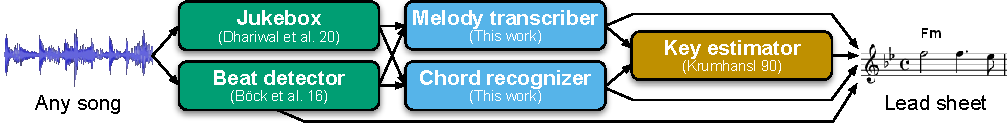
\includegraphics[width=\linewidth]{figs/sheetsage.pdf}
    \caption{Inference procedure for Sheet Sage, our proposed system which transcribes any Western music audio into lead sheets (scores which depict melody as notes and harmony as chord names). The green, blue, and yellow boxes respectively take audio, features, and symbolic music data as input. Green boxes are modules that we built as part of this work---both are Transformers~\cite{vaswani2017attention} trained on their respective tasks using audio features from Jukebox~\cite{dhariwal2020jukebox} and data from \hooktheory~\cite{hooktheory}.}
    \label{fig:sheet_sage}
    \vspace{-3mm}
\end{figure*}

Overall, using representations from \jukebox{} as input features results in stronger melody transcription performance than using either representations from \mtthree{} or conventional handcrafted features. 
Representations from both \mtthree{} and \jukebox{} outperform conventional handcrafted features, 
implying that both pre-training strategies are helpful for melody transcription. 
Note that these two pre-training approaches are compared holistically---these models differ on several axes 
(number of parameters, 
pre-training data semantics, 
pre-training task), 
and thus it is impossible to disentangle the individual contributions of these different factors without retraining the models. 

Qualitatively speaking, there is a noticeable difference in performance across the three different input features which correlates with quantitative performance (see~\cref{sound_examples} for sound examples). 
Using representations from \jukebox{} tends to result in fewer wrong notes than the other features, and substantially reduces the number of egregiously wrong notes (e.g.,~notes outside of the key signature). 
Representations from \jukebox{} also appear to aid in the detection of more nuanced rhythmic patterns. 
Moreover, using handcrafted features will often result in several repeated onsets during a longer sustained melody note---in contrast, using representations from \jukebox{} appears to mitigate this failure mode.

Different features also appear to complement one another to a degree. 
The strongest performance overall is obtained by combining all three features, though the improvement over \jukebox{} alone is marginal. 
The practical downsides of combining all features outweigh the marginal benefits---running both pre-trained models effectively doubles the overall runtime, and the models have incompatible software dependencies. 
Hence, in the remainder of this paper we focus on models trained on individual features.

\vspace{-1mm}
\subsection{Comparison to melody transcription baselines}
\label{sec:exp2}

We compare overall performance of our proposed melody transcription approach to several baselines. 
We evaluate all methods on a small subset of $10$ songs from RWC-MDB~\cite{goto2002rwc,goto2003rwc,goto2004development}, 
another dataset which includes melody transcription labels. 
We chose this specific subset in an effort to compare to early DSP-based work on melody transcription---none of the early approaches~\cite{paiva2004auditory,paiva2005detection,ryynanen2008automatic,weil2009automatic} shared code, however~\cite{ryynanen2008automatic} shared melody transcriptions for this $10$-song subset.

In addition to~\cite{ryynanen2008automatic}, we also compare to a baseline which applies a note segmentation heuristic~\cite{salamon2015midi} to a melody extraction algorithm~\cite{salamon2014melody}. 
We additionally compare to \mtthree{} in a zero-shot fashion---this model was not trained on melody transcription but was trained on some tasks which incorporate vocal transcription. 
Finally, because the vocals often carry the melody in popular music, we compare to a baseline of running the Tony~\cite{mauch2015computer} monophonic transcription software on source-separated vocals isolated with Spleeter~\cite{hennequin2020spleeter}. 
Because this approach will only work for vocals, we also separately report performance on a subset of our evaluation set where the vocals represent the melody. 
Scores for all methods and baselines appear in~\Cref{tab:rwc_ryy}. 

Overall, our approach to training Transformers with features from \jukebox{} significantly outperforms the strongest baseline in both the vocals-only and unrestricted settings (${p < 0.01}$ using a two-sided t-test for paired samples). 
Qualitatively speaking, the stronger baselines produce transcriptions where a reasonable proportion of the notes are the correct pitches, but they have poor rhythmic consistency with respect to the ground truth. 
In contrast, our best model produces the correct pitches more often and with a higher degree of rhythmic consistency.

\vspace{-2mm}
\section{Sheet Sage}
\label{sec:sheetsage}

%\pl{make it clear that this is just a demo (bonus) we built and aren't going to evaluate it rigorously just to set expectations?}
As a bonus demo, 
here we describe \sheetsage, a system we built to automatically convert music audio into lead sheets (see footnote on first page for examples), powered by our \jukebox-based melody transcription model. 
In Western music, a piece can often be characterized by its melody and harmony. 
When engraved as a lead sheet---a musical score containing the melody as notes on a staff and the harmony as chord names---melody and harmony can be readily interpreted by musicians, enabling recognizable performances of existing pieces. 
Hence, for some music, a lead sheet represents the essence of its underlying composition.
Existing services like Chordify~\cite{de2014chordify} can already detect a subset of the information needed to produce lead sheets (specifically, chords, beats, and keys) for broad music audio. 
However, despite past research efforts~\cite{ryynanen2008automatic,weil2009automatic}, no user-facing service yet exists which can convert broad music audio into lead sheets, presumably due to the poor performance of existing melody transcription systems.

To build \sheetsage, we also train a \jukebox-based chord recognition model on the \hooktheory{} data, using the same methodology that we propose for melody transcription (we simply replace the target vocabulary of onset pitches with one containing chord labels).
%We use an extended chord vocabulary consisting of $96$ chord labels (major, minor, 7, maj7, m7, sus, dim, aug for each of the 12 pitch classes).
Passing audio through our \jukebox{}-based melody transcription and chord recognition models results in a score like format containing raw note names and chord labels per sixteenth note. 
Engraving this information as a lead sheet requires additional information: the key signature and the time signature. 
We estimate the former using the Krumhansl-Schmuckler algorithm~\cite{krumhansl1990cognitive,temperley1999key}, which takes the symbolic melody and chord information as input. 
For the latter, we use \madmom~\cite{bock2016madmom,bock2016joint}. 
Finally, we engrave a lead sheet using Lilypond~\cite{nienhuys2003lilypond}. 
See~\Cref{fig:sheet_sage} for a full schematic.

Subjectively speaking, \sheetsage{} often produces high-quality lead sheets, especially for the chorus and verse segments of pop music which have more prominent melodies. 
Performance is fairly robust across styles and instruments, even those which are less represented in the training data---one user reported particularly strong success on Bollywood music. 
However, the system occasionally struggles, especially with quieter vocals, layered harmonies, unusual time signatures, or poor intonation. 
\sheetsage{} is also limited to fixed time and key signatures due to limitations of its downbeat detection and key estimation modules.

\section{Conclusion}

We present a new method and dataset which together improve melody transcription on broad music audio. 
Our method benefits from the rich representations learned by generative models pre-trained on broad audio. 
This suggests that further improvement in melody transcription may be possible without additional melody transcription data, i.e.,~by scaling up or otherwise improving the pre-training procedure. 
By releasing our models and dataset, we hope to spark renewed interest for melody transcription in the MIR community, which in turn may reduce the gap between human perception and machine recognition of a fundamental aspect of music.
\john{Consider making a broader parting statement than this?}

\section{Ethical considerations}

Our definition of melody transcription incorporates equal temperament, a Western-centric tuning system. 
This could lead to disparate treatment of non equal-tempered music, e.g.,~if recommender systems were to incorporate transcriptions.
%a streaming service were to use melody transcriptions for recommendations. 
We therefore advocate for the deployment of transcription only in contexts where users are self selecting music to listen or play along to. 
%, and that recommendation algorithms instead incorporate lower-level features such as \fnot. 
Additionally, transcription may be used to create training data for generation. 
As with any work on generation, there are risks of plagiarism and displacement of musicians. 
We recommend that any work on generation closely examine plagiarism within their system. 
Due to the incomplete nature of a melody, we argue that melody generation tools are more likely to be incorporated into a musician's workflow (see~\cite{huang2020ai} for examples) rather than displace them.

%\section{Acknowledgements}

% JohnH for helpful discussions
% Annie for engraving advice
% Sam Ainsworth for JAX help through JohnT
% Megha Srivastava for being an enthusiastic user
% Nelson Liu for being an enthusiastic user and helpful discussions
% Rodrigo Castellon for helpful discussions

\bibliography{main}

\end{document}

